% This procedure has three sub-procedures in each paragraph below.
\paragraph{The Simple Transition Path}
We first collect the loop headers $\loopl(c) \subseteq \lvar(c)$ from a program $c$, which is the set of all program points corresponding to the loop headers.
% in program $c$,
Then we collect all the \emph{simple transition path}s, $\tpath$ from its abstract transition graph as follows.
\begin{defn}[Simple Transition Path]
 \label{def:tpath}
A \emph{simple transition path}
$\tpath$ for the program $c$, is either a simple cyclic path
%, which has the same start- and end-point
or a simple path having either different while loop headers, the program entrance or exit as its start- and end-point
without visiting any loop header inside the path.
\\
Formally, a path $l_0 \xrightarrow{dc_0} l_1 \xrightarrow{dc_1} \ldots l_n \in \paths(\absG(c))$ with the
vertices $(l_0, \ldots, l_n)$ and the edges $(e_1, \ldots, e_n)$, where $l_i \in \absV(c)$ and $e_i = (l_{i - 1}, dc_i, l_{i}) \in \absE(c)$ for every $i = 0, \ldots, n$
%
is a \emph{simple transition path} if and only if it satisfies,
\begin{itemize}
 \item $l_i \neq l_j$ for every $i = 0, \ldots, n$ and $j = 0, \ldots, {n - 1}$,
 \item $l_0$ is either the program point of a loop header or the program entrance ($l_0 = 0$),
 i.e., $l_0 \in \loopl(c) \cup \{ 0 \}$
 \item and $l_n$ is either the program point of a loop header or the program exit ($l_n = \lex$),
 i.e., $l_0 \in \loopl(c) \cup \{ \lex \}$,
 \item and $l_i \notin \loopl(c) \cup \{ 0, \lex \}$ for every $i = 1, \ldots, n-1$.
\end{itemize}
\end{defn}
Each $\tpath$ is loop-free and interleaving-free corresponding to a path in the flatten program in Definition~4.1 in \cite{GulwaniJK09}.
% contains only the edges of atomic assignment or guard transitions, which
For example in Figure~\ref{fig:relatedNestedWhileOdd-overview}(b), the $1 \to 2 \to 8 \to 1$ is a \emph{simple transition path}.
However, $1 \to 2 \to 3 \to 4 \to 5 \to 4 \to 6 \to 7 \to 1$ is not a \emph{simple transition path} because it is not simple.
Also, $1 \to 2 \to 3 \to 4 \to 6 \to 7 \to 1$ is not a \emph{simple transition path} because it visits a loop header $4$ inside the path. $1 \to 2 \to 3$ isn't either because its end-point isn't a loop header.

\paragraph{Program Rewriting}
Then we rewrite the program $c$ by rearranging all \emph{simple transition path}s as the syntax in \cite{GulwaniJK09} and preserves the same semantics in Algorithm~\ref{alg:alg-refine_rewrite} in Appendices~\ref{apdx:alg-rewrite}.
% We first collect all the \emph{simple transition path}s as the algorithm input. 
The algorithm takes the set of all $\tpath$ as the input and initializes each candidate with a
$\tpath$.
In iterating, it generates new candidates by composing and deletes the used ones until stabilized.
%
The corresponding rewritten program in Figure~\ref{fig:relatedNestedWhileOdd-overview} is
$ 
\tpath_0; \rpchoose{\rprepeat(\tpath_1; 4:\rprepeat(\tpath_3); \tpath_2),\rprepeat(\tpath_4) }; \tpath_5
$.

\paragraph{Program Refinement}
We implement the algorithm REFINE from paper~\cite{GulwaniJK09} in this step which takes the rewritten program $c$ as input and returns the
refined program $\rprog$. We denote by $\kw{enclosed}(\rprog, \tpath)$ the innermost loop where $\tpath$ is located in $\rprog$.
The $\rprog$ at the bottom of Figure~\ref{fig:relatedNestedWhileOdd-overview} where we can find two interleaving patterns.
The two loop paths are alternatively executing after each other in the two patterns and
 $4:\rprepeat(\tpath_3) = \kw{enclosed}(\rprog, \tpath_3)$.

 We use another example from the benchmark set of~\cite{GulwaniJK09} to show the necessity of the \emph{path refinement}. It has a two paths loop
 with different \emph{reachability-bound}s on the locations of different paths.
 We denote by $\absevent \in \rprog$ that $\absevent$ is an edge on  an $\tpath'$ in $\rprog$.
 %
Given $n \geq m$,
the expected \emph{reachability-bound} for the locations $4$ and $5$ on the$\ethen$branch is $m \times \lfloor\frac{n}{m}\rfloor$
while for locations on the other branch, $2$ and $3$ is $(m + 1) \times \lfloor\frac{n}{m}\rfloor + 1$. 
The best state-of-art bound analysis
gives the same \emph{reachability-bound}, $n + \lfloor\frac{n}{m}\rfloor$ for all the locations within the loop $L_2$.
    { \footnotesize
    \begin{figure}
    \centering
    %
    \begin{subfigure}{.27\textwidth}
        $
        \begin{array}{l}
          \kw{twoPathsWhile}(n, m) \triangleq \\
        \clabel{ \assign{i}{n} }^{0} ;
        \clabel{ \assign{j}{0} }^{1} ; \\
        L_2:    \ewhile ~ \clabel{i > 0}^{2} ~ \edo ~ \\
            \qquad \big(
              \eif(\clabel{j < m}^{3}, \\
              \qquad \ethen  \clabel{\assign{j}{j + 1}}^{4}; \\
              \qquad \qquad \clabel{\assign{i}{i - 1}}^{5},\\
              \qquad \eelse \clabel{\assign{j}{0}}^{6});
              \big)
            \end{array}
            $
\vspace{-0.2cm}
\caption{}
\end{subfigure}
\begin{subfigure}{.71\textwidth}
\begin{subfigure}{.67\textwidth}
\begin{centering}
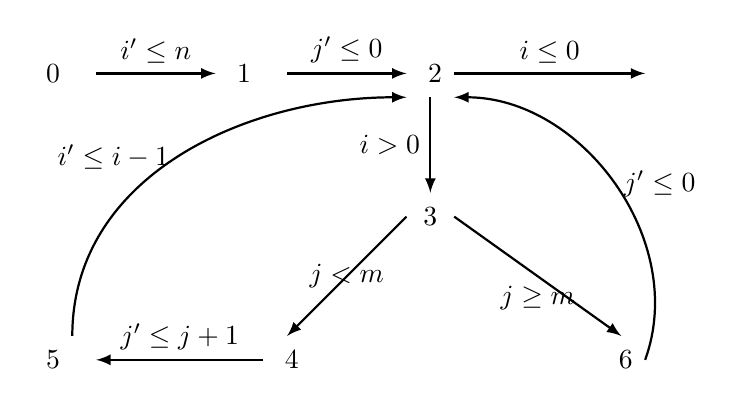
\begin{tikzpicture}[scale=\textwidth/20cm,samples=200]
    \draw[] (-8, 10) circle (0pt) node{{ $0$}};
    \draw[] (-4, 10) circle (0pt) node{{ $1$}};
    \draw[] (0, 10) circle (0pt) node{{ $2$}};
    \draw[] (0, 7) circle (0pt) node{{$3$}};
    \draw[] (-3, 4) circle (0pt) node{{ $4$}};
    \draw[] (-8, 4) circle (0pt) node{{ $5$}};
    \draw[] (4, 4) circle (0pt) node{{ $6$}};
    % Counter Variables
    \draw[] (5, 10) circle (0pt) node {\textbf{$\lex$}};
    %
    % Control Flow Edges:
    \draw[ thick, -latex] (-7, 10)  -- node [above] {$i' \leq n$}(-4.5, 10);
    \draw[ thick, -latex] (-3, 10)  -- node [above] {$j' \leq 0$}(-0.5, 10);
    \draw[ thick, -latex] (0, 9.5)  -- node [left] {$i > 0$} (0, 7.5) ;
    \draw[ thick, -latex] (0.5, 7)  -- node [below] {$ j \geq m $}  (4, 4.5);
    \draw[ thick, -latex] (-7.5, 4.5)  to  [out=90,in=180]  node [left] {$i' \leq i - 1$ }(-0.5, 9.5);
    \draw[ thick, -latex] (4.5, 4)  to  [out=70,in=0]   node [right] {$j' \leq 0 $}(0.5, 9.5);
    \draw[ thick, -latex]  (-0.5, 7) -- node  {$j < m$}  (-3, 4.5) ;
    \draw[ thick, -latex]  (-3.5, 4) -- node [above] {$j' \leq j + 1$}  (-7, 4) ;
    \draw[ thick, -latex] (0.5, 10)  -- node [above] {$i \leq 0$}  (4.5, 10);
  \end{tikzpicture}
        \caption{}
\end{centering}
\end{subfigure}
{\small
\begin{subfigure}{.3\textwidth}
\begin{centering}
        $\tpath_0 = 0 \to 1 \to 2$ \\
        $\tpath_2 = 2 \to 3 \to 6 \to 2$ \\ 
        $\tpath_1 = 2 \to 3 \to 4 \to 5 \to 2$ \\
        $\tpath_3 = 2 \to \lex$
        \caption{}
\end{centering}
\end{subfigure}
}
{\small
\begin{subfigure}{.8\textwidth}
\begin{centering}
    $
    \tpath_0 ; 
    \rpchoose{2: \rprepeat(\rprepeat(\tpath_1); \tpath_2), 
    2: \rprepeat(\tpath_1)}; \tpath_3.
    $
\end{centering}
\end{subfigure}
}
\end{subfigure}
\vspace{-0.2cm}
\caption{
    (a) The two paths loop example,
    (b) the Abstract Transition Graph for $\kw{twoPathsWhile}(n, m)$,
    (c) the Simple Transition Paths of $\kw{twoPathsWhile}(n, m)$.}
    \vspace{-0.5cm}
        \label{fig:whileTwoCounters-overview}
    \end{figure}
    }



To know the bounds for locations on different branches of a loop, 
it is necessary to know the alternative iteration patterns of the two paths.
So over its abstract transition graph generated by Section~\ref{sec:progabs} as Figure~\ref{fig:whileTwoCounters-overview}(b), we collect all its simple transition path as in Figure~\ref{fig:whileTwoCounters-overview}(c).
Through loop refinement, we explicate the interleaving between paths and
% using the control-flow refinement technique from~\cite{GulwaniJK09} and 
transform the loop into the refined program $\rprog$ as the bottom part of Figure~\ref{fig:whileTwoCounters-overview}.
From this refined program, we can explicitly tell two possible path interleaving patterns.
In the first one, $\tpath_2$ will be executed after all the iterations of $\tpath_1$ are done, and in the second one,
only the first loop path $\tpath_1$ will iterate.
Then the following computation based on this refined program can compute more accurate \emph{reachability-bound}s.

